%%% License: Creative Commons Attribution Share Alike 4.0 (see https://creativecommons.org/licenses/by-sa/4.0/)

\documentclass[english,10pt
%,handout
,aspectratio=169
]{beamer}
%%% License: Creative Commons Attribution Share Alike 4.0 (see https://creativecommons.org/licenses/by-sa/4.0/)

\DeclareGraphicsExtensions{.eps, .pdf,.png,.jpg,.mps,}
\usetheme{reMedian}
\usepackage{parskip}
\makeatother

\renewcommand{\baselinestretch}{1.1} 

\usepackage{amsmath, amssymb, amsfonts, amsthm}
\usepackage{enumerate}
%\usepackage{enumitem}
\usepackage{hyperref}
\usepackage{url}
\usepackage{bbm}
\usepackage{color}

\usepackage{tikz}
\usepackage{tikzscale}
\newcommand*\circled[1]{\tikz[baseline=(char.base)]{
		\node[shape=circle,draw, inner sep=-20pt] (char) {#1};}}
\usetikzlibrary{automata,positioning}
\usetikzlibrary{decorations.pathreplacing}
\usepackage{pgfplots}
\usepgfplotslibrary{fillbetween}
\usepackage{graphicx}

\usepackage{setspace}
\thinmuskip=1mu
\medmuskip=1mu 
\thickmuskip=1mu 


\usecolortheme{default}
\usepackage{verbatim}
\usepackage[normalem]{ulem}

\usepackage{apptools}
\AtAppendix{
	\setbeamertemplate{frame numbering}[none]
}
\usepackage{natbib}


% red strikeout
\newcommand\soutred{\bgroup\markoverwith
	{\textcolor{red}{\rule[0.55ex]{2pt}{0.8pt}}}\ULon}



% To use LyX frames from old version:
\def\lyxframeend{} % In case there is a superfluous frame end
\long\def\lyxframe#1{\@lyxframe#1\@lyxframestop}%
\def\@lyxframe{\@ifnextchar<{\@@lyxframe}{\@@lyxframe<*>}}%
\def\@@lyxframe<#1>{\@ifnextchar[{\@@@lyxframe<#1>}{\@@@lyxframe<#1>[]}}
\def\@@@lyxframe<#1>[{\@ifnextchar<{\@@@@@lyxframe<#1>[}{\@@@@lyxframe<#1>[<*>][}}
\def\@@@@@lyxframe<#1>[#2]{\@ifnextchar[{\@@@@lyxframe<#1>[#2]}{\@@@@lyxframe<#1>[#2][]}}
\long\def\@@@@lyxframe<#1>[#2][#3]#4\@lyxframestop#5\lyxframeend{%
	\frame<#1>[#2][#3]{\frametitle{#4}#5}}


\title{Mechanism Design}

\subtitle{0: Introduction}

\author{Egor Starkov}

\date{K{\o}benhavns Unversitet \\
	Fall 2021}


\begin{document}
	\AtBeginSection[]{
		\frame<beamer>{
			\frametitle{This slide deck:}
			\tableofcontents[currentsection,currentsubsection]
	}}
	\frame[plain]{\titlepage}


\section{What is mechanism design?}

\begin{frame}{What is Game Theory?}
\begin{center}
	Economic agents interact with each other.
	\pause
	
	$\Downarrow$
	
	What is the outcome? 
	
	How is it shaped by environment?
\end{center}
\end{frame}


\begin{frame}{What is Mechanism Design?}
\begin{center}
	\pause[2] 
	How to shape the environment to achieve it?
	
	$\Uparrow$
	
	\pause[1]
	There is some desirable outcome.
\end{center}
\end{frame}


\begin{frame}{Example 1}
	\begin{columns}
		\begin{column}{0.6\linewidth}
			{\setstretch{1.3}\\
				You want to sell an apartment. What is the best way to do so?
				\begin{itemize}
					\item Market conditions change; potential buyers come and go. How long should you wait?
					\item Run an auction or bargain with each buyer?
					\item Reveal all house issues truthfully or let buyers find them?
				\end{itemize}
			}
		\end{column}
		\begin{column}{0.4\linewidth}
			\pause[1]
			\includegraphics<handout:0>[width=\linewidth]{pics/M0/8tallet}
		\end{column}
	\end{columns}
\end{frame}


\begin{frame}{Example 2}
\begin{columns}
	\begin{column}{0.6\linewidth}
		{\setstretch{1.3}\\
			A country needs to elect a new president. How to organize the election?
			\begin{itemize}
				\item How many candidates, how many rounds, etc?
				\item Turnout to physical voting is typically low. Should you allow online voting?
				\item Should you allow buying votes (voting with money)?
			\end{itemize}
		}
	\end{column}
	\begin{column}{0.4\linewidth}
		\pause[1]
		\includegraphics<handout:0>[width=\linewidth]{pics/M0/debate}
	\end{column}
\end{columns}
\end{frame}


\begin{frame}{Example 3}
\begin{columns}
	\begin{column}{0.6\linewidth}
		{\setstretch{1.3}\\
			Is it possible to design an effective decentralized currency? (Think cryptocurrency)
			\begin{itemize}
				\item Where does money come from and how to avoid counterfeits?
				\item If money is digital, how to avoid double spending?
				\item If someone needs to process transactions, how to design their rewards?
			\end{itemize}
		}
	\end{column}
	\begin{column}{0.4\linewidth}
		\pause[1]
		\includegraphics<handout:0>[width=\linewidth]{pics/M0/coins}
	\end{column}
\end{columns}
\end{frame}


\begin{frame}{Who plays the players?}
	\begin{columns}
		\begin{column}{0.6\linewidth}
			{\setstretch{1.3}
				\begin{itemize}
					\pause
					\item Can see the ``designer'' as yet another player
					\item Moves first and determines what others can do
					\item But has a \emph{very large} action set
				\end{itemize}
			}
		\end{column}
		\begin{column}{0.4\linewidth}
			\pause[1]
			\includegraphics<handout:0>[width=\linewidth]{pics/M0/housewins}
		\end{column}
	\end{columns}
\end{frame}


\begin{frame}{This course}
	What can you expect?
	\begin{itemize}
		\item overview of main results over past 40 years
		\item not that much from the frontier
		\item plenty of math! (brace yourselves) (also see math review on absalon)
		\item intuition and economics behind the models
		\item models are abstract but are applicable to a \textbf{lot of} areas (industrial organization, political economy, taxation, auctions\ldots{})
		\item see course description for more details on what exactly you learn
	\end{itemize}
\end{frame}


\begin{frame}{Related courses at KU}
\begin{itemize}
	\item Contract theory, Auctions
	\item Economics of organization, Corporate Finance, Industrial organization
	\item Other courses in which applications of mechanism design appear:
	\begin{itemize}
		\item Public finance/Taxation
		\item Political economy
		\item Monetary
		\item Labor
		\item \ldots{}
	\end{itemize}
\end{itemize}
\end{frame}





\section{Logistics}

\begin{frame}{Hi}
\begin{itemize}
	\item Egor Starkov
	\item \texttt{egor.starkov@econ.ku.dk} or absalon inbox
	\item Research interests: information economics, dynamic games, communication
	\item Office: 26.1.13
	\item Questions: email/absalon, before/after class
\end{itemize}
\end{frame}


\begin{frame}{Logistics}
\begin{itemize}
	\item Weekly lectures (except Fall break -- week \#42)
	\begin{itemize}
		\item Fri, 12:15-15:00, CSS 2.1.12
	\end{itemize}
	
	\pause
	\item Mandatory assignment:
	\begin{itemize}
		\item ``Make your own problem'' -- find an interesting real-world setting and analyze it using the machinery from the class
		\item groups of up to 4 are allowed
		\item deadline: some time in November?
	\end{itemize}
	
	\pause
	\item Final exam:
	\begin{itemize}
		\item 24hrs take home (individual, no groups)
		\item Convert problems from text to math; solve them and explain intuition
	\end{itemize}

	\pause
	\item Research module: contact me if you would like to do it
\end{itemize}
\end{frame}


\begin{frame}{Covid-specific stuff}
	\begin{itemize}
		\item Idea is to have as much physical teaching as possible
		\item But will have Zoom broadcasts until further notice
	\end{itemize}
\end{frame}


\begin{frame}{Materials}
	\begin{itemize}
		\item Intended workflow: 
		\begin{enumerate}
			\item We start a topic in class
			\item \uline{You watch video-lectures at home} during the week (+read textbook, slides, whatever's necessary)
			\item We discuss any questions in class and solve some problems
			\item You will have more problems to practice at home
		\end{enumerate}
		\pause
		\item Suggestion: organize into groups. Watch lectures in groups. Discuss problems in groups.
		\pause
		\item In class I use whiteboard+slides. Slides on absalon include some of the whiteboard parts.
		\begin{itemize}
			\item I'll try to upload slides in advance, but they might be edited and updated afterwards
		\end{itemize}
	\end{itemize}
\end{frame}


\begin{frame}{References}
	This course is a compilation of many books, papers, courses; does not follow any single one too closely. But the following four references cover about 90\% of the class.
	\begin{itemize}
		\item textbooks:
		\begin{description}
			\item[B\"{o}rgers] Tilman B\"{o}rgers. An introduction to the theory of mechanism design. Oxford University Press, 2015.
			\item[RS] Roth \& Sotomayor. Two-Sided Matching: A Study in Game-Theoretic Modeling and Analysis. Cambridge: Cambridge University Press. 1990.
		\end{description}
		\item survey papers:
		\begin{description}
			\item[B\&V] Bergemann, Dirk, and Juuso Välimäki. ``Dynamic mechanism design: An introduction.'' Journal of Economic Literature 57.2 (2019): 235-74.
			\item[B\&M] Bergemann, Dirk, and Stephen Morris. ``Information design: A unified perspective.'' Journal of Economic Literature 57.1 (2019): 44-95. 
		\end{description}
	\end{itemize}
\end{frame}


\begin{frame}{References}
	alternative textbooks:
	\begin{description}
		\item[Diamantaras] Diamantaras, Cardamone, Campbell, Deacle, and Delgado. A toolbox for economic design. Macmillan, 2009.
		\item[MWG] Mas-Colell,  Whinston, Green. Microeconomic theory. Oxford University Press, 1995. 
	\end{description}
\end{frame}


\begin{frame}{References}
	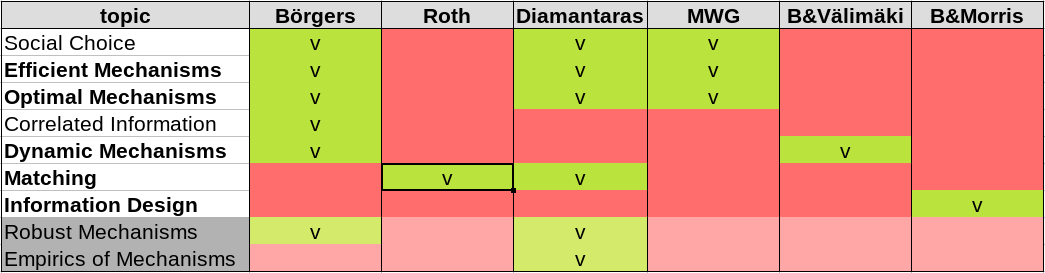
\includegraphics[width=\textwidth]{pics/M0/sources}
	\\
	see reading list on absalon for details
\end{frame}


\begin{frame}{References}
	In the end:
	\begin{itemize}
		\item I suggest getting B{\"o}rgers' textbook. It is not necessary, but might be useful.
		\item Diamantaras or MWG are okay alternatives.
		\item I do \textbf{not} recommend getting Roth \& Sotomayor textbook unless you are really interested in the topic of matching. Promise the slides will be sufficient for that part of the class.
	\end{itemize}
\end{frame}


\section{First taste}

\begin{frame}{Example: Environment}
	Let's go back to the apartment sale example and try to tackle the simplest version of it: one buyer, one seller, one item on sale.
	\pause
	
	\begin{itemize}
		\item \structure<2>{Seller}: likes money, has \textbf{known} valuation $\structure<2>{\bar{\theta}} \in [0,1]$ for the item
		\begin{itemize}[<4>]
			\item \structure<4>{utility}: $u_0(k,t) = t - \bar{\theta} k$
		\end{itemize}
		\item \structure<2>{Buyer}: likes money, has \textbf{private} valuation $\structure<2>{\theta} \in [0,1]$ for the item
		\begin{itemize}[<4>]
			\item \structure<4>{utility}: $u_1(k,t,\theta) = \theta k - t$
		\end{itemize}
		\pause
		\item let \structure<3>{$k \in \{0,1\}$} denote whether the sale occurs
		\item let \structure<3>{$t \in \mathbb{R}_+$} denote the price of the sale (or any other transfer between the buyer and the seller)
	\end{itemize}
\end{frame}


\begin{frame}{Example: Environment comments}
	\begin{itemize}
		\item $k$ and $t$ constitute the \textbf{outcome} (e.g., $(k,t)=(1,0.5)$ = ``apt sold for 0.5 moneys''). Outcome will, almost always, depend on the buyer's valuation $\theta$. So the object we are interested in is the outcome \emph{function} $(k(\theta), t(\theta))$.
		
		\item For simplicity, allow payments $t$ to be made even if the item is not sold (otherwise better to define $u_0(k,t) = (t - \bar{\theta}) k$ and $u_1(k,t,\theta) = k (\theta - t)$). Also, $t$ that the buyer pays is the same $t$ that the seller receives -- there are no sales taxes, agent commissions, etc.
		
		\item Both players are assumed to be risk-neutral (otherwise utilities are not linear in $t$, which is mildly inconvenient). Obviously, we also ignore everything that does not fit the von Neumann-Morgenstern expected utility model (including ambiguity/disappointment/loss aversion, regret, prospect theory, etc).
	\end{itemize}
\end{frame}


\begin{frame}{Example: Efficient mechanism}
	Before we go to seller's revenue maximization, suppose policymaker is the designer, wants to facilitate \textbf{efficient trade}.
	
	\begin{itemize}
		\item What does ``efficient trade'' mean?
		\pause
		Efficient = maximizes social surplus: for any $\theta$,
		\begin{align*}
			(k^*(\theta),t^*(\theta)) &\in \arg \max_{k(\theta),t(\theta)} \left\{ u_0(k,t) + u_1(k,t,\theta) \right\}
			\\
			&= \arg \max_{k(\theta),t(\theta)} \left\{ t(\theta) - \bar{\theta} k(\theta) + \theta k(\theta) - t(\theta) \right\}
			\\
			&= \arg \max_{k(\theta),t(\theta)} \left\{ k(\theta) \cdot (\theta - \bar{\theta})  \right\}
		\end{align*}
		\pause
		so $k^*(\theta) = \mathbb{I} \{ \theta > \bar{\theta} \}$ (=trade whenever the buyer values the item more), and $t^*(\theta)$ can be anything.
		\pause
		\item This can be implemented by setting a fixed price $t = \bar{\theta}$. Buyer will then obviously buy if and only if $\theta > \bar{\theta}$.
	\end{itemize}
\end{frame}


\begin{frame}{Example: Efficient mechanism comments}
	\begin{itemize}
		\item The irrelevance of price comes from linearity of utilities in $t$, both agents having the same sensitivity to $t$, and the designer assigning same weight to both agents' utilities.
		\begin{itemize}
			\item This will be our approach for most of the course -- everyone is equal, so redistribution does not matter; the only goal of transfers is to provide incentives.
			\item In principle, you can factor equality into the problem by adjusting the designer's objective function appropriately.
		\end{itemize}
	\end{itemize}
\end{frame}


\begin{frame}{Example: Optimal mechanism}
	Now back to the original question: what is the sale mechanism that \textbf{maximizes seller's revenue}?
	\pause
	
	\begin{itemize}
		\item First, what is the realm of all possible mechanisms? What are we choosing from?
		\pause
		\begin{itemize}
			\item Any mechanism produces some outcomes $k,t$
			\item ...though these depend on $\theta$, so they are actually functions $k(\theta),t(\theta)$.
			\item Given these functions, we can always propose a ``direct mechanism'': ``buyer reports $\theta$ to the mechanism, and respective outcomes are implemented.
		\end{itemize}
		
		\pause
		\item But can we choose any pair of functions $k(\theta),t(\theta)$? Or are there any restrictions we should impose?
		\pause
		\begin{itemize}
			\item Well, the idea is for the buyer to report $\theta$ truthfully. So the mechanism should be such that it is optimal for the buyer to report truthfully \alert{$\leftarrow$ ``Incentive compatibility''}
			\item Also, buyer should be willing to participate in the mechanism, as opposed to walking away -- so should get higher utility than what can get by walking away (zero) \alert{$\leftarrow$ ``Individual rationality''}
		\end{itemize}
	\end{itemize}
\end{frame}


\begin{frame}{Example: Optimal mechanism}
	Now back to the original question: what is the sale mechanism that \textbf{maximizes seller's revenue}?
	
	So in the end we get the following problem:
	\begin{align*}
		\max_{k(\cdot),t(\cdot)} & \mathbb{E}_\theta \left[ t(\theta) - \bar{\theta} k(\theta) \right]
		\\
		\text{s.t. (IC): } & \theta k(\theta) - t(\theta) \geq \theta k(\hat{\theta}) - t(\hat{\theta}) \text{ for all } \theta,\hat{\theta}
		\\
		\text{(IR): } &\theta k(\theta) - t(\theta) \geq 0 \text{ for all } \theta
	\end{align*}
	\pause
	This is almost a standard maximization problem. Except we're maximizing over \uline{functions}, as opposed to one or two numbers... And there is an \uline{infinite} number of constraints...
	\pause
	Want to know how to solve this? Tune in next week for more mechanism design!
\end{frame}


\begin{frame}{For next week}
	\begin{enumerate}
		\item Watch lectures 2.1 (`What is a mechanism?') and 2.2 (`Dominant strategy implementation')
	\end{enumerate}
\end{frame}


\end{document}